\documentclass[10pt,twocolumn]{article}
% ═══ PRP-V127 PLATFORM — v5 EN (guardian-gated, two-tier G0) ═══
% Source of truth: manuscript_EN_v5.md (48 claims; guardian R0-R3 PASS, 0 BLOCKED)
\usepackage[margin=1.9cm,columnsep=0.7cm]{geometry}
\usepackage{lmodern}
\usepackage{mathptmx}
\usepackage{graphicx,booktabs,amsmath,amssymb}
\usepackage[hang,flushmargin]{footmisc}
\usepackage{caption}\captionsetup{font=small,labelfont=bf}
\usepackage{titlesec}\titleformat{\section}{\large\bfseries}{\thesection}{0.6em}{}
\usepackage{fancyhdr}\pagestyle{fancy}\fancyhf{}
\fancyfoot[C]{\tiny Preprint v5EN --- full audit: github.com/camillanapoles/quest003-prion-v127 (48 claims · 33 sources · guardian R0-R3 · data-tier labels [SIM]/[ORGANOID]/[MOUSE]/[HUMAN])}
\fancyfoot[R]{\thepage}\renewcommand{\headrulewidth}{0pt}
\usepackage{xcolor}
\newcommand{\rtnote}[1]{\ensuremath{^{\textcolor{gray}{\scriptsize\texttt{#1}}}}}
\setlength{\footnotesep}{2pt}\setlength{\skip\footins}{6pt}
\usepackage{microtype}

\title{\bfseries PrP-V127 as a Modular Antiprion Platform: Audited Review, Quantitative Transport Design, Humanized In-Silico Predictions, and a Pre-Registered Organoid Gate for Creutzfeldt--Jakob Disease}
\author{\normalsize Open Prion \& Molecular Engineering Consortium\thanks{Corresponding: Camilla N. (conceptualization, methodology, software, investigation, writing --- CRediT in repository \texttt{authorship.json}). AI agents assisted literature curation, code, drafting and hostile-review harnessing under continuous human supervision; every citation and number verified against sources by the accountable author; AI is not an author (SW-S01/03). Full audit trail incl.\ claim-level traceability and the guardian harness: \texttt{github.com/camillanapoles/quest003-prion-v127} (branch \texttt{paper-v5}).}}
\date{}

\begin{document}\maketitle

\begin{abstract}\small
Prion diseases are universally fatal with no approved therapy. We report a pre-registered translational design thesis converting the naturally selected human variant PrP-V127 into a quantitatively designed therapeutic platform for CJD, evolved through documented evidence-triggered revisions (\S1.2). \textbf{Methods:} (i) provenance-verified agent-assisted audit ($\approx$90 searches; 60 findings, 9 blocks; 33 audited sources; corrected citation record incl.\ a retracted trial). (ii) Self-tested advection--diffusion--reaction transport solver (mass conservation 100\%; Thiele error 0.5\%) yielding three falsifiable design rules: ring spacing 8--12\,mm; hydrogel mesh $\xi\ge5r_p$; LNP-mRNA redosing $\le$7\,d. (iii) Hierarchical Bayesian frame over 10 analogues incl.\ the six historical failures: P(clinical slowing)$=$5.0\% [0.4--13.6] empirical \emph{vs} 30--45\% design-conditional (both lenses labeled). (iv) Humanized in-silico model: the open stochastic kernel of Fornara/Igel (iScience 2024), fidelity-corrected and capped by V127$\Delta$GPI as saturable substrate competition, clock-calibrated to human organoid anchors (1 unit $=$ 144\,d). \textbf{Results:} containment threshold $\theta^{*}=0.333$ (front 2.83$\to$0.82\,mm at $\kappa{=}2$; near-extinction at $\kappa{=}32$) and unprompted MV2$>$MV1 hierarchy consistency. \textbf{Gate architecture (two-tier, declared):} the in-silico gate \textbf{G0-sim [SIM] is executed and passed} (T1/T2/T3 machine-audited); the wet-lab organoid gate \textbf{G0-wet [ORGANOID]} is fully specified pending production. Computational findings are used as results in their own epistemic tier: they do not substitute validation and do not block continuation --- on the contrary, they stimulate agile, assertive R\&D consistent with scientific methodology. \textbf{Locked prediction (release v1.0):} $\theta_{\text{measured}}<0.33\Rightarrow$ containment; readouts 90--120\,d. From this revision onward all outputs carry data-tier labels ([SIM]/[ORGANOID]/[MOUSE]/[HUMAN]). Every regulatory pillar maps to an approved category (nusinersen; tofersen/NfL; 2026 Parkinson grafts; tafamidis): the program requests a conjunction of precedents, with the conjunction itself declared as the novel risk.
\end{abstract}

\begin{figure*}[t]\centering

\includegraphics[width=\textwidth]{figs/fig1_scientific_map.png}
\caption{\textbf{How this program was executed.} Four methodological phases (audit $\to$ transport physics $\to$ probability $\to$ humanized in-silico) feeding the evidence harness (33 sources, 48 claims, four validators at zero errors, guardian R0--R3) which locks the pre-registered G0 prediction.}\label{fig:map}
\end{figure*}

\section{Introduction}
Human prion diseases are rapidly progressive and universally fatal; sCJD survival is 6--8 months; six candidates failed clinically. The G127V polymorphism, positively selected during kuru, confers complete resistance when homozygous in transgenic mice with potent dose-dependent dominant-negative inhibition; heterozygotes remain vCJD-infectable (partial shield $=$ permeable). In 2026, recombinant anchorless V127 retained trans dominant-negative activity with persistence after expression ceases, and systemic AAV delivery extended survival $\sim$50 days in rodents; the structural basis is established ($\beta2$--$\alpha2$ loop restriction, H-bond dimers). The mechanism is validated at four levels --- population genetics, transgenic mouse, cell culture, gene-therapy proof-of-concept. What was missing is the \emph{engineering}: delivery modality, dose, placement, timing, and a decision architecture that spends laboratory resources only where models cannot answer. This manuscript reports the complete pre-wet-lab program, fully audited and guardian-gated.

\emph{Populations.} Primary: presymptomatic genetic carriers (E200K/D178N; Brazilian kindreds since 2007) --- therapeutic window of years, autologous manufacture feasible. Sporadic CJD: exclusively via acellular LNP-mRNA under compassionate use after organoid validation (single intrathecal dose transduces 29.6\% of neurons / 38.1\% of astrocytes in rodents).

\subsection{Program evolution audit}
The program began as a pre-clinical review of one cell-therapy protocol and became a quantitative design thesis through documented, evidence-triggered revisions --- every pivot anchored to a refutation in-repo, none by preference: SVZ ``central factory'' refuted (quiescent human niche that itself replicates prions) $\to$ cortical deposits $+$ 8--12\,mm ring; CRISPR biallelic shield demoted (heterozygote permeability; trans activity without anchor) $\to$ secretory graft (A5) $+$ LNP-mRNA (A7); permanent factory $\to$ redosing $\le$7\,d; 6-arm gate $\to$ 8-arm gate (+A7, +A8 pentosan-polysulfate published control). Invariants across revisions: the V127 dominant-negative containment thesis; population-first E200K-Brazil; pre-registered gates with kill-switches; audit-first epistemology; the organoid gate as decisive experiment.

\section{Methods}
\subsection{Agent-assisted audit (provenance-verified)}
Structured blocks ($\approx$90 searches $\to$ 9 evidence tables, 60 findings; $\sim$30 papers in depth; verification tiers [FT]/[ABS]/[AUDIT]/[CODE]/[RUN]). External documents' references audited individually (one batch of 19: 11 correct, 3 duplicates, 1 non-scientific, 1 wrong link). A retracted Neurotherapeutics trial still circulating as evidence is excluded by rule; minocycline additionally confounds the NfL endpoint (3.5$\times$ plasma, 5.7$\times$ CSF) with no survival benefit. Search reproducibility: queries being consolidated into \texttt{search\_log.md} (declared gap).

\subsection{Transport solver (WS-7) [SIM]}
ADR in heterogeneous porous medium; finite volumes (2D, $192^2$, explicit Euler):
\begin{equation}\partial(\alpha c)/\partial t=\nabla\!\cdot\!(D_{\text{eff}}\nabla c)-\nabla\!\cdot\!(\mathbf{v}c)+S(\mathbf{x})-k_{\text{eff}}c\end{equation}
Parameters (Table 1): $\alpha{=}0.20$, $\lambda{=}1.8$ (in-vivo integrative optical imaging); $D_0{=}1.25{\times}10^{-10}$\,m$^2$/s (Stokes--Einstein, $R_h{\approx}2.5$\,nm, $\sim$30\,kDa) $\Rightarrow D_{\text{eff}}{=}3.86{\times}10^{-11}$\,m$^2$/s; $k_{\text{eff}}$ swept $10^{-6}$--$10^{-5}$\,s$^{-1}$ (central $3{\times}10^{-6}\approx0.26$\,d$^{-1}$; nucleated-polymerization kinetics). Darcy flow; spongiform cysts $\kappa\times50$. Self-tests: mass conservation 100.0\%; Thiele error 0.5\% ($\ell{=}3.59$\,mm). \emph{Verification scope:} numerics verified; validation against published distribution profiles is future work --- rules stated as ratios, robust to absolute-concentration error. \emph{Formal definition:} $\theta\equiv(1+\kappa c_{\text{peak}})^{-1}\in(0,1]$: the fraction of maximal replication activity remaining where the secretion field peaks; containment declared at front radius $<$50\% of baseline (T3). \emph{Order-of-magnitude $\kappa$-anchoring (illustrative assumptions; closed by arm A6):} $c(r)\approx(Q/4\pi D_{\text{eff}}r)e^{-r/\ell}$ with illustrative inputs $10^5$ cells $\times$ 10\,pg/cell/day gives $c(1\,\text{mm})\approx0.8$\,\textmu M; across the plausible range $\approx$0.1--1\,\textmu M --- the range where culture dominant-negative effects are observed. $\kappa{=}2$--4 $\leftrightarrow$ roughly 0.1--1\,\textmu M interstitial V127$\Delta$GPI (illustrative, not a measured secretion estimate).

\subsection{Bayesian frame (WS-8) [SIM]}
Hierarchical Beta--Binomial over 10 analogues, $w_j\propto$ similarity$^2$ (mechanism, vector, population, endpoint); six failures as negative analogue (0/6); ION717 partially informative; organoid predictive validity $\approx$0.8 (PDO proxy, declared); $2{\times}10^5$ draws. Outputs pre-registered: P(G0-wet informative-go)$=$36.6\% [14.6--60.5]; P(slowing)$=$5.0\% [0.4--13.6] empirical \emph{vs} 30--45\% design-conditional; a third structural lens (62\%) archived, not blended. Declarations: failure sources outside the E-registry pending elevation (queued); weights single-rater (sensitivity queued).

\subsection{Humanized in-silico model (WS-9) [SIM]}
\emph{Kernel:} Fornara/Igel stochastic reaction--diffusion (open code, Zenodo 11093945) ported to deterministic mean-field (96$^2$, $dt{=}5{\times}10^{-4}$) with two fidelity-critical corrections decoded from \texttt{findreac}: the $s{+}1$ channel is autocatalytic ($C{\to}2C$) and the cross-reaction is fragmentation. Logistic saturation $C/(C+C_{50})$ bounds mean-field autocatalysis (documented port limitation). \emph{Capping (this work):} freeS $=(1+\kappa c_{V127})^2$ enters all templating terms (two-participant competitive saturation). \emph{Humanization:} global time rescaling --- relative rates remain murine; clock matched to organoid anchors (clearance 25--28\,dpi; de-novo 35\,dpi; titers MV2 $2.13{\times}10^5$ \emph{vs} MV1 $1.69{\times}10^3$ SD50/mg at 169\,dpi; PrP-res only in MV2) $\Rightarrow$ doubling $\approx$12.1\,d; 1 unit $=$ 144\,d; seeds differ by the $126\times$ ratio. \emph{Acceptance tiers:} T1/T2 minimal screening; \textbf{T3 informative} $=$ front $<$50\% baseline at $\kappa\le8$ with monotone radial gradient --- satisfied at $\kappa{=}2$ (0.82\,mm $=$ 29\% of 2.83\,mm); T3 is a post-hoc analysis-tier label on pre-registered outputs (declared).

\subsection{Pre-registration and reproducibility}
Gate architecture is two-tiered: G0-sim (computational, executed and passed) and G0-wet (organoid, specified). All predictions locked at repository release v1.0 before any wet-lab data exist; code, parameters, outputs (JSON + figures) archived in-repo. G0-wet: 8 arms (mock; disease; unedited cell; membrane-V127; \emph{secretory graft}; recombinant protein; LNP-mRNA; PPS positive control), $n{=}8$/arm, primary readout proximal/distal PrP-res gradient. \textbf{Statistical analysis plan:} per-arm Welch t-test vs disease control, $\alpha{=}0.05$ Holm-corrected across 5 informative comparisons; n$=$8 detects $\Delta\ge$50\% at power $\approx$80\% (CV$\sim$30\%), escalating to n$=$12; blinded PrP-res quantification and per-batch randomization frozen in the execution checklist; batch/line stratification given published organoid variance (MV2 SD $\approx$77\% of mean). Locked $\theta$ prediction refers to MV2-like challenge; MM1 is a future claim conditional on anchors. \textbf{Program-level kill criterion:} no containment gradient at any dose AND $\theta_{\text{obs}}>0.33$ in all informative arms $\Rightarrow$ program terminates; negative result published.

\subsection{Recursive hostile-review harness (guardian gate)}
Deterministic hostile-review harness (in-repo, stdlib-only, offline): (R0) structural drift --- claim/evidence/manifest binding, adjacent traceability markers, LaTeX--manuscript number divergence; (R1) hostile checklist M1--M8/m1--m10 as testable patterns $+$ per-claim-kind question batteries $+$ unbound-decimal detection; (R2) recursion on amendments (illustrative estimates must not carry evidence tags; PT/EN claim parity; locked predictions cite immutable anchors); (R3) epistemic interrogation (operational $\theta$, statistical plan, blinding, failure-source binding, preprint dependence, conjunction risk, search logs, localization, sensitivity sweeps, redosing immunogenicity, canon, G0-sim declaration, tier labeling, [no-year] thesis, anticipatory-method innovation). Gate $=$ zero BLOCKED; reports published with the manuscript. Manuscript-quality gate, not peer review: it certifies consistency and traceability; scientific validity is testable only by G0-wet.

\subsection{Operational definition of $\theta_{\text{obs}}$}
The locked prediction requires an estimator ($\theta$ is a model quantity): (i) PrP-res radial profiles quantified by a blinded scorer; (ii) per-organoid $\theta_{\text{obs}}$ by fitting the humanized $\kappa$-grid to the measured gradient (least squares, simulation normalization); (iii) per-arm median with bootstrap 90\% CI; (iv) comparison to 0.333 with pre-declared decision margin; (v) estimator code, grid and objective committed before unblinding. Without this freeze the locked prediction would be circular; the estimator is therefore part of the pre-registration.

\section{Results}
\subsection{Audit}
Four-layer validated core; five recurring field design errors corrected (NSC$\to$microglia lineage impossibility; prion-replicating quiescent SVZ; others), each replaced by evidence-compatible branches (iPSC-microglia co-graft; slow-release deposits; LNP-mRNA). Pivotal single-source claims (kuru selection; organoid anchors) flagged with no independent replication known at audit date.

\subsection{Design rules [SIM]}
R1 spacing 8--12\,mm (halo radius 4--6\,mm); R2 hydrogel $\xi\ge5r_p\Rightarrow D_{\text{gel}}/D_0\ge0.7$; R3 redosing $\le$7\,d (trough $\ge$56\% of peak); steady state $\sim$4\,d; wave-vs-shield containment shell 4.2--9.5\,mm (Fig.~2).

\subsection{Probabilities [SIM]}
As \S2.3; both lenses labeled; structural lens archived unblended.

\subsection{Humanized predictions [SIM]}
$\theta^{*}{=}0.333$; monotone to near-extinction ($\kappa{=}32$: 0.70\,mm; biomass 2.1$\times$ seed); one run $\approx$24 months of tissue disease. Mechanism of the humanized shift: the global rescale lengthens replication per unit of diffusive transport --- a scale interaction, not a re-fit. \textbf{Emergent qualitative consistency (declared confound):} the $126\times$ seeding ratio reproduces MV2$>$MV1 unfitted (MV2-like contained 0.78\,mm; MV1-like 0.69\,mm at $\kappa{=}4$; Fig.~3); hierarchy \emph{consistency}, not proof of subtype-specific kinetics; same-mass control queued.

\subsection{Gate status declaration: computational continuation}
\textbf{Objective of this stage, declared in full:} to carry the research to the end of its arc within the simulated environment --- real, parametrized data at every step (published murine kinetics; in-vivo human transport parameters; human organoid anchors; audited review) --- and to harvest the complete set of results simulation can yield: design rules, containment threshold, subtype behavior, probability frames, estimator specification, queued sensitivity map. Three declared reasons: final in-silico results (i) maximize the informative yield and assertiveness of every future validation gate; (ii) generate precise quantitative expectations that attract further research, partnership and replication; (iii) exercise in full the methodological innovation of this thesis --- computational evaluation as an engine of research continuation (predictability and information anticipation; \S4.1). The thesis objective is stated \textbf{without a calendar year}: defined by results --- the complete simulation harvest [SIM], then gate-by-gate validation [ORGANOID]$\to$[MOUSE]$\to$[HUMAN]; phase durations are planning estimates, never promises. G0-sim is \textbf{executed and passed} (T1/T2/T3, emergent consistency, humanized clock; pre-registered, timestamped, machine-audited). Validity basis: systematic review $+$ published murine-parameterized kernel $+$ human organoid anchors --- materially stronger than the traditional route (no prior antiprion candidate had a quantitative delivery model, a corrected review layer, or pre-registered falsification thresholds). G0-wet is specified and pending production; its pending status \textbf{does not impede continuation}: sweeps (freeS exponent, $C_{50}$, same-mass control), $\theta_{\text{obs}}$ estimator development and rule refinement proceed now, each raising the informative yield of the future wet-lab gate (P$=$36.6\% prices this). The relationship between tiers is deliberately constructive: computational findings are \textbf{used as results in their own epistemic tier} --- they do not substitute biological validation and equally do not block continuation; on the contrary they \textbf{stimulate agile, assertive research and development consistent with scientific methodology}. \textbf{Scope (guardian-enforced):} G0-sim licenses continuation (design, resources, protocol freeze, estimator); it does not license biological-validation claims or clinical inference; validation remains explicit, necessary and non-substitutable. \textbf{Data-tier labeling (continuity rule):} the gate ladder is named by medium --- G0-sim [SIM] (executed) $\to$ G0-wet [ORGANOID] (specified) $\to$ G1 [MOUSE] (conditional) $\to$ G2 [HUMAN] (conditional); every forthcoming output carries its tier tag; until G0-wet exists, all new program data are [SIM] --- parametrized, audited, pre-registered; never presented as measured. \textbf{Thesis architecture (two parts joined at the G0 junction):} \emph{Part 1 (pre-G0)} --- the research arc of this manuscript: audited review, findings, parametrized simulation, design rules, probability frames, benefits --- culminating in the G0-sim harvest [SIM] and the fully specified G0-wet gate. \emph{Part 2 (post-G0): the continuity thesis} --- research and validation that use the parametrized simulation data as their working substrate ($\theta_{\text{obs}}$ consumes the pre-computed $\kappa$-grid; arms, doses and placements chosen by the design rules; measured data re-parameterize the models), operationalizing predictability and information anticipation for therapeutic design: deciding what to measure, where, and at what dose before any wet-lab resource is spent. Neither part is systematically sustainable without the other: Part 1 alone would be an unexercised design; Part 2 alone, unguided experimentation. The junction is G0 --- which is why its declaration, estimator, statistical plan and kill criteria are specified in full before any wet-lab exists.

\begin{table*}[t]\centering\small
\caption{\textbf{Consolidated parameters with provenance} (full registry: \texttt{consistency\_manifest.json}, 39 numeric facts).}
\begin{tabular}{llp{8.5cm}}
\toprule
Parameter & Value & Source / tier \\
\midrule
ECS fraction $\alpha$ / tortuosity $\lambda$ & 0.20 / 1.8 & in-vivo IOI (published [ORGANOID-era literature]) \\
$D_0$ (30\,kDa anchorless) & $1.25{\times}10^{-10}$\,m$^2$/s & Stokes--Einstein [SIM param from published physicochem.] \\
$D_{\text{eff}}$ & $3.86{\times}10^{-11}$\,m$^2$/s & $D_0/\lambda^2$ [SIM] \\
$k_{\text{eff}}$ & $10^{-6}$--$10^{-5}$\,s$^{-1}$ (0.26\,d$^{-1}$ central) & nucleated polymerization [SIM sweep] \\
Thiele length $\ell$ & 3.59\,mm & $\sqrt{D_{\text{eff}}/k}$; numeric err 0.5\% [SIM] \\
R1 ring spacing & 8--12\,mm & WS-7 [SIM] \\
R2 hydrogel mesh & $\xi\ge5r_p\Rightarrow D_{\text{gel}}/D_0\ge0.7$ & WS-7 [SIM] $+$ published HA scaffolds \\
R3 redosing & $\le$7\,d (trough $\ge$56\%) & WS-7 pulse-train [SIM] \\
LNP transduction (IT dose) & 29.6\% neurons / 38.1\% astrocytes & published (rodent) \\
Human doubling / sim unit & 12.1\,d / 144\,d & derived from organoid anchors [SIM] \\
MV2 / MV1 titers @169\,dpi & $2.13(\pm1.63){\times}10^5$ / $1.69(\pm0.70){\times}10^3$ SD50/mg & published organoid data \\
Titer ratio & 126$\times$ & derived from published data \\
$\theta^{*}$ / front at $\kappa{=}2$ & 0.333 / 0.82\,mm (baseline 2.83) & WS-9 humanized [SIM] \\
P(G0-wet go) / P(slowing) & 36.6\% / 5.0\% (empirical); 30--45\% conditional & WS-8 [SIM] \\
Self-tests & mass 100\%; Thiele 0.5\% & WS-7 [SIM] \\
Illustrative $\kappa$ anchor & $\kappa$2--4 $\leftrightarrow$ 0.1--1\,\textmu M & declared assumptions; closed by A6 \\
\bottomrule
\end{tabular}
\end{table*}

\begin{figure}[t]\centering
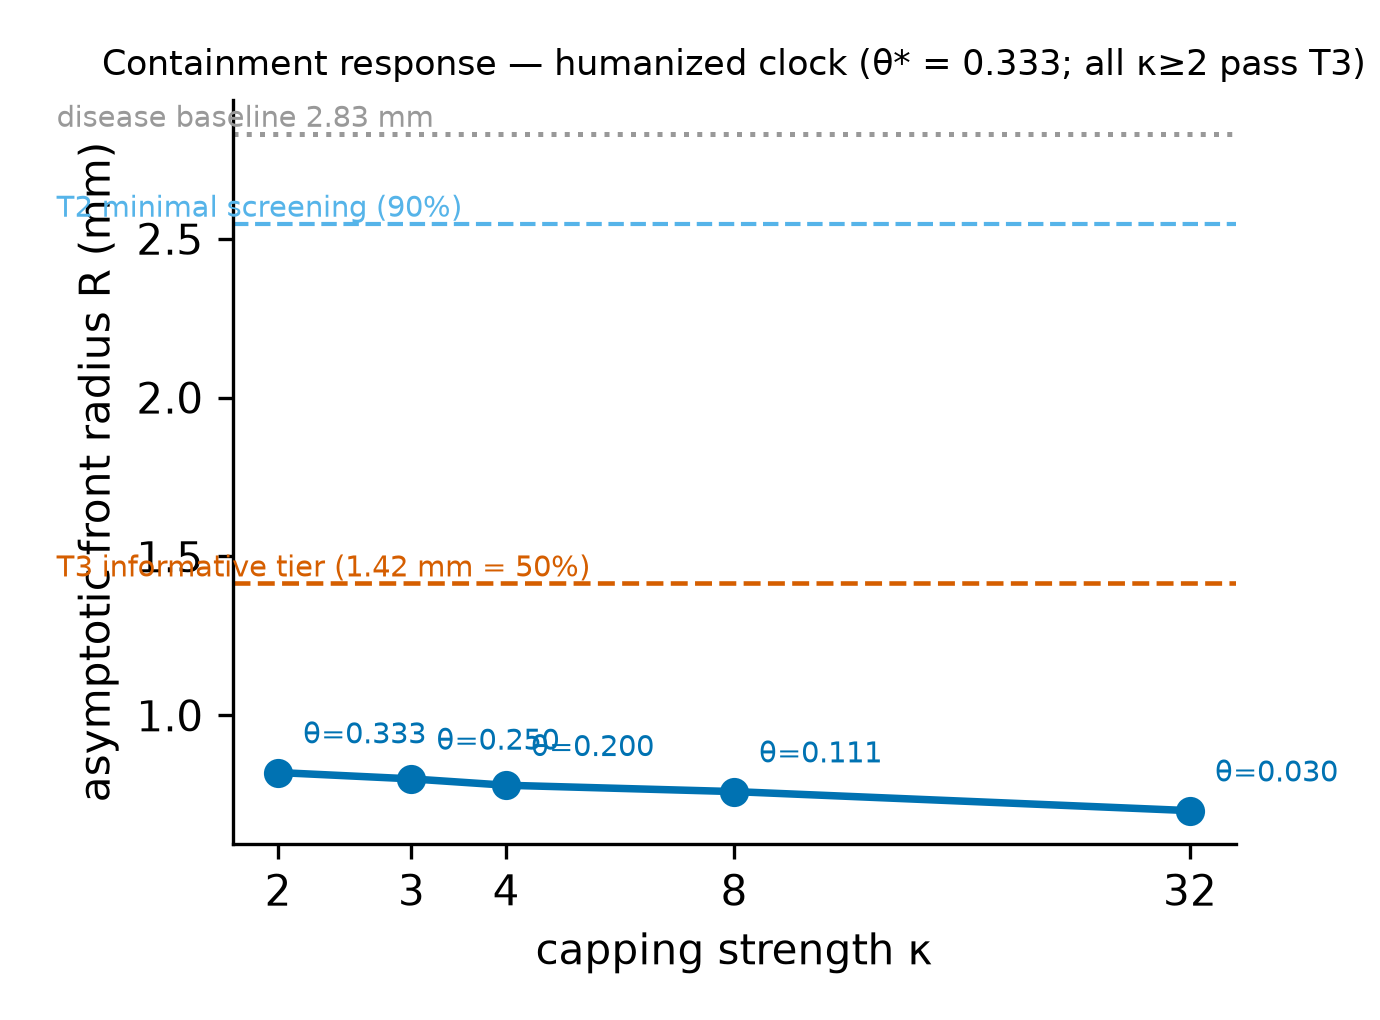
\includegraphics[width=\columnwidth]{figs/fig2_theta_response.png}
\caption{\textbf{Containment response [SIM].} Asymptotic front radius vs capping strength $\kappa$ (humanized clock). T2 minimal screening and the informative T3 tier annotated; all $\kappa\ge2$ pass T3. Values from the archived run JSON.}\label{fig:theta}
\end{figure}

\begin{figure}[t]\centering
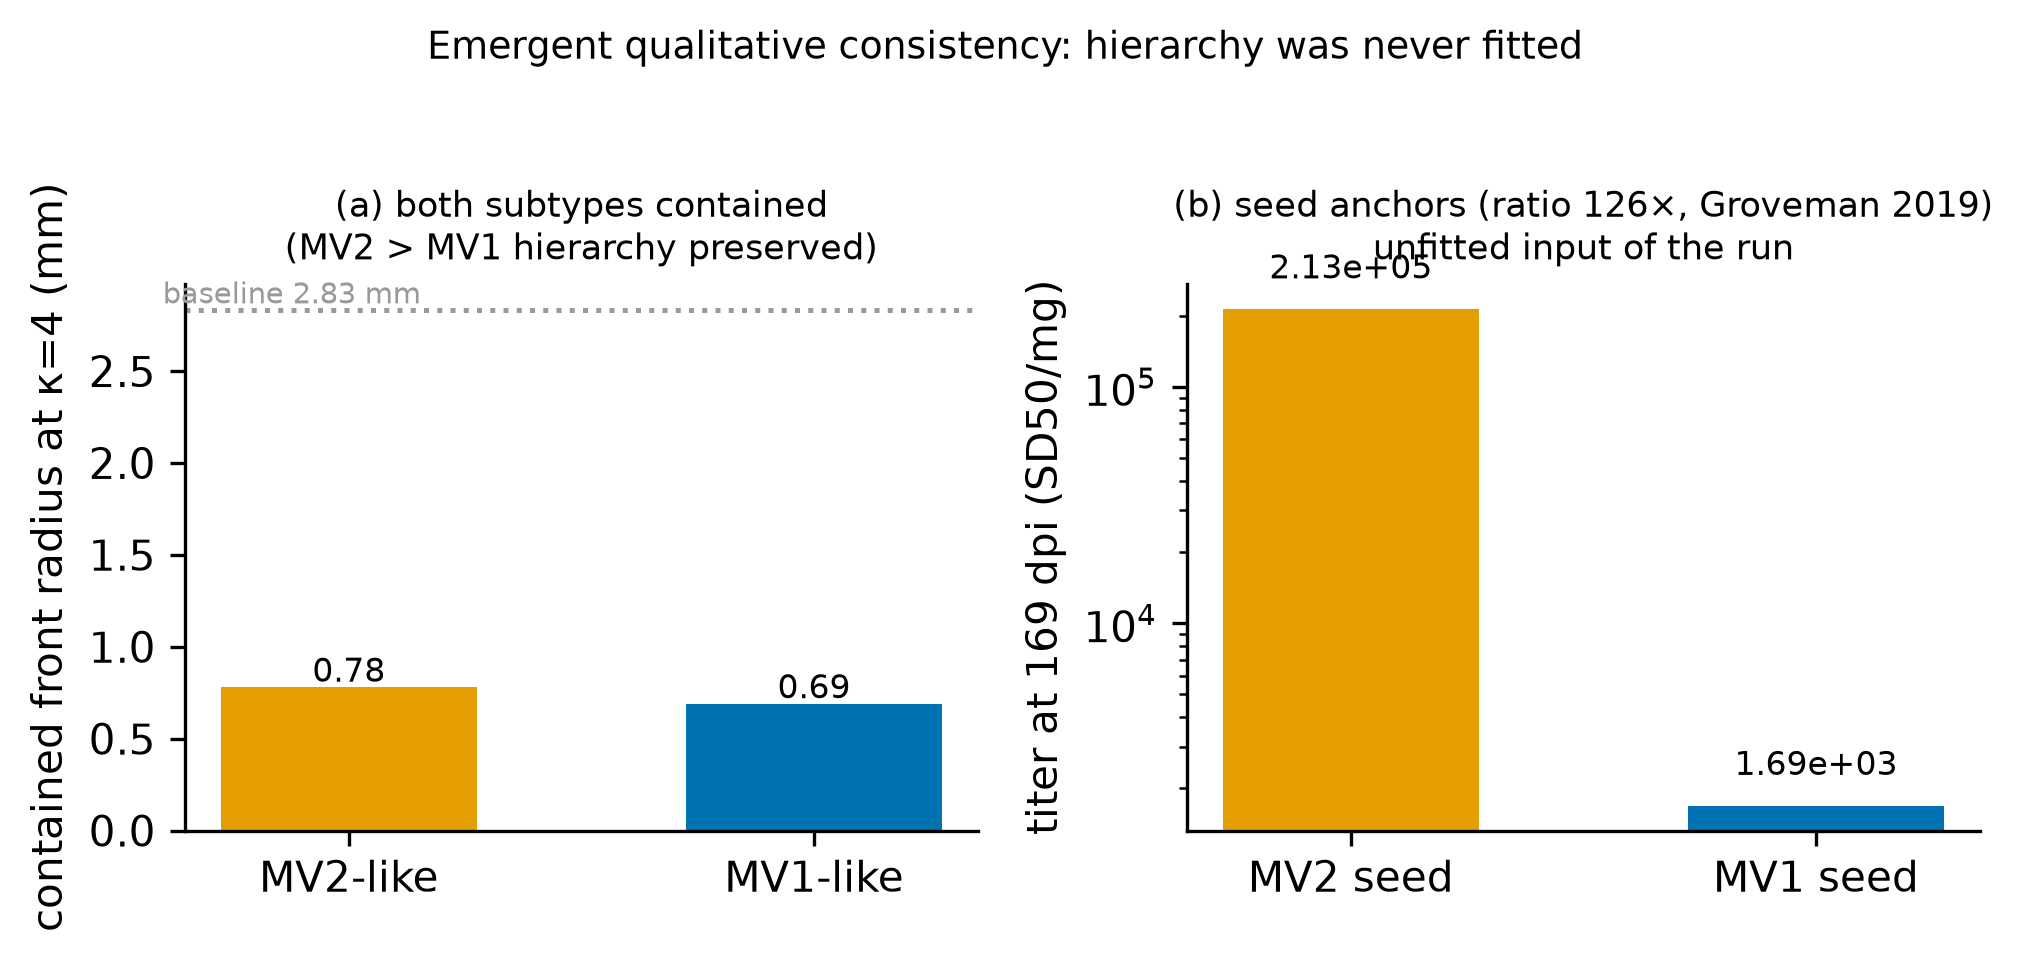
\includegraphics[width=\columnwidth]{figs/fig3_subtypes.png}
\caption{\textbf{Emergent subtype consistency [SIM].} (a) Both MV2-like and MV1-like seeds contained at $\kappa{=}4$; hierarchy preserved. (b) Seed anchors ($126\times$, published organoid titers) --- unfitted input of the run.}\label{fig:sub}
\end{figure}

\section{Discussion}
\subsection{What this program adds}
To prion science: a quantitative delivery-and-dose calculus no prior candidate possessed; a corrected citation record; pre-registered falsifiable predictions with a 10-month, $\sim$\$100--150k kill-or-advance assay (planning estimate; decomposition queued). To methodology: an executable template of agent-assisted, provenance-verified translational planning (audit $\to$ physics $\to$ Bayes $\to$ simulation $\to$ pre-registered gate) with a recursive hostile-review gate keeping manuscript, registries and rendered edition from drifting. The discovery model is the audited arc itself --- evolution-validated variant $\to$ quantitative containment design $\to$ pre-registered falsifiable gate --- transferable independent of therapeutic outcome. \textbf{Methodological innovation:} computational evaluation as research continuation joins the family of anticipation methods (systematic review/meta-analysis; physics-based modeling; Bayesian forecasting; in-silico trials) as a fully documented instance whose explicit purpose is predictability and information anticipation for therapeutic design. The epistemic mode is that of theoretical physics: estimates precede, direct, and hold until superseded by measurement --- halting the computational program until laboratory confirmation would reduce, not increase, knowledge production; published evidence is used directly, while the undocumented enters as pre-declared methodology.

\subsection{Transferability (hypothesis-generating)}
Alzheimer and Parkinson spread by templated misfolding along stereotyped routes. The platform calculus is mechanism-agnostic; prion disease is the fastest, cheapest-to-read instance ($>$50M patients in the class). One asymmetry declared: the calculus transfers, the agent does not --- V127's advantage is a naturally selected protective variant; for A$\beta$/$\alpha$-synuclein no equivalent exists (existence uncertainty beyond engineering uncertainty).

\subsection{Regulatory geometry}
Chronic intrathecal redosing (nusinersen); accelerated approval via biomarker (tofersen, NfL); human brain cell grafts (2026 Parkinson); dominant native-state stabilization (tafamidis); substrate lowering (ASO/RNAi). Declared logical limit: a precedent for each pillar is not a precedent for the conjunction --- the combination is itself the novel regulatory object; weakest pillar: the secretory anti-prion graft (Parkinson 2026 engrafts progenitors, not a secreting biofactory). Competitive position (declared): substrate-reduction ASOs (ION717) are 3--5 years ahead in pipeline and partially deplete native PrP; V127 dominant-negative containment preserves native PrP --- complementarity, not superiority; both may combine.

\section{Limitations}
(1) $\kappa\to$concentration order-of-magnitude only (closed by A6). (2) Mean-field port; stochastic extinctions/strain diversity absent; heterologous-seeding recruitment would make $\theta^{*}$ a lower bound (optional co-aggregation readout). (3) $C_{50}$ was a stability choice --- closed by sweep [SIM]: threshold insensitive over a tenfold range. (4) MV1/MV2 anchors only; MM1 unpublished; humanization $=$ global time rescale, rates murine. (5) Detection floor $10^2$ assumed. (6) Healthy-tissue transport parameters; synthetic cyst $\kappa\times50$ pending poroelastography. (7) Analogue weights single-rater. (8) No wet-lab data yet: all \S3 outputs are [SIM] predictions. (9) Murine$\to$human transfer via dimensional $\theta$ assumed until G0-wet. (10) Immunogenicity/clearance of the construct uncharacterized; repeated-dose LNP immunogenicity (anti-PEG, complement) uncharacterized intrathecally --- A7 includes local inflammatory markers. (11) T3 post-hoc label on pre-registered outputs. (12) Hierarchy confound resolved [SIM]: in the v4 kernel subtype $\equiv$ seed mass --- seed-mass-driven by construction. (13) Preprint-dependence of the anchorless-trans layer (two 2026 preprints; monitored). (14) Ring localization unsolved for sporadic translation (presymptomatic genetic carriers reduce to stereotyped anatomy). (15) Cost estimate not decomposed.

\section{Ethics, governance, declarations}
Population-first design; DSMB with pre-specified stop; prion biosafety (single-use coaxial cannula; WHO 134\,\textdegree C/NaOH; autopsy containment); LGPD privacy; containment/slowing endpoints only. Probabilistic figures are design estimates, not clinical predictions; coverage reaching patient organizations should carry that framing. Equity: Brazilian E200K kindreds anchor the hypothesis; access planning is part of governance. \textbf{Funding:} none (volunteer consortium; Colab free tier). \textbf{Conflicts:} none; no patent filings. \textbf{AI disclosure:} as title footnote. \textbf{Data/code:} everything public (MIT/CC-BY), incl.\ the guardian harness, knowledge canon, G0 unlock dossier and gate-tier labels. \textbf{Authorship:} Camilla N. (corresponding); CRediT and accountability in-repo.

\section*{References (33 audited sources; author--year)}
\small
Asante EA, et al. Nature 522:478 (2015). Mead S, et al. NEJM 361:2056 (2009). Gatdula JRP, et al. bioRxiv 2026.02.17.703887 (preprint). Zerbes T, et al. PMC13041815 (2026, preprint). Hosszu LP, et al. Commun Biol 3:580 (2020). Zheng Z, et al. Sci Rep 8:11458 (2018). Groveman BR, et al. Acta Neuropathol 137:987 (2019). Groveman BR, et al. Sci Rep 11:5160 (2021). Fornara B, Igel A, et al. iScience (2024; Zenodo 11093945). Thorne RG, Nicholson C. PNAS 103:8217 (2006). Masel J, et al. Biophys Chem 77:139 (1999). Williams K, et al. Stem Cell Res Ther (2023). Rela\~no-Gin\'es A, et al. PLoS Pathog 9:e1003485 (2013). Ginhoux F, et al. Science 330:841 (2010). Sorrells SF, et al. Nature 558:253 (2018). Abud EM, et al. Neuron 94:278 (2017). Han X, et al. PNAS 116:10441 (2019). Hu X, et al. Nat Biotechnol 42:807 (2024). Xue Y, et al. Adv Mater (2025). Liang Y, et al. Biomaterials 34:3948 (2013). Shah SZA, et al. Neurotherapeutics (retracted 2020). Cheng S, et al. Sci Rep 5:10535 (2015). Gentile JE, et al. UK DRI (2024). Smid J, et al. Dement Neuropsychol (2007). Stopschinski BE, Diamond ML. Lancet Neurol (2017). Jucker M, Walker LC. Nature (2018). FDA tofersen accelerated approval (2023). FDA nusinersen (2016). Lund University Parkinson cell-transplant trial (2026). Consortium software/dataset E030--E033 (2026, in-repo). \emph{Identifiers and verification tiers: repository \texttt{source\_manifest.json}; full claim--evidence traceability: \texttt{claims.csv} (48 claims) and the guardian traceability appendix.}

\end{document}
